\documentclass{report}
\usepackage{pdfpages}
\usepackage{enumerate}
\usepackage[a4paper, total={6in, 8in}]{geometry}
\graphicspath{ {images/} }

\title{Homework \# 1}
\author{Bhumsitt "Bose" Pramuanpornsatid}
\date{\today}

\begin{document}

\maketitle

\section*{Question 1}
(10 points) A teacher gives 5 students a multiple choice test, in which each problem is worth 1 point and there is no penalty with negative points. The median and mean scores turn out to be 9 and 10 points, respectively.

\begin{enumerate}[(a)]
    \item What is the minimum of the possible top scores?
    \item What is the maximum of the possible top score?
    \item What is the minimum of the possible standard deviations?
    \item What is the maximum of the possible standard deviations?
\end{enumerate}

\subsection*{Answer}
As the mean is given to be 10 points and there are 5 students. The total score of all students is $5*10=50$ points.
\begin{enumerate}[(a)]
    \item The minimum top scores is 12. This case is possible when we arrange the set of score to be $\{9, 9, 9, 11, 12\}$. The median is 9, and the mean is 10 which satisfy the question. By setting the score of the first 2 students to equal the median. The sum of the last 2 students must be 23. The combination of 11 and 12 will result in the minimum of the top scores and sum up to 23. Therefore, 12 is the minimum of the possible top scores.
    \item The maximum top scores is 32. This case is possible when we arrange the set of score to be $\{0, 0, 9, 9, 32\}$. The median is 9, and the mean is 10 which satisfy the question. By setting the score of the first 2 students to equal 0. The sum of the last 2 students must be 41. The combination of 9 and 32 will result in the maximum of the top scores and sum up to 41. Therefore, 32 is the maximum of the possible top scores.
    \item The minimum possible standard deviation is 1.265. This case is possible when we arrange the set of score to have the least variance $\{9, 9, 9, 9, 14\}$. 
    \newline Calculation of standard deviation: $\sqrt{\frac{1+1+1+1+4}{5}}=\sqrt{1.6}\approx1.265$
    \item The maximum possible standard deviation is 11.713. This case is possible when we arrange the set of score to have the most variance $\{0, 0, 9, 9, 32\}$.
    \newline Calculation of standard deviation: $\sqrt{\frac{100+100+1+1+484}{5}}=\sqrt{137.2}\approx11.713$
\end{enumerate}

\newpage
\section*{Question 2}
(10 points) Let $\{x_i\}$ be a dataset consisting of $N$ real numbers, $x_1,...,x_N$.
\begin{enumerate}[(a)]
    \item Prove from definitions or proved properties in the textboook that the standardized data set $\{\hat{x_i}\}$ that is derived from $\{\hat{x_i}\}$ has mean = 0 and standard deviation = 1
    \item If the median of data set $\{\hat{x_i}\}$ is -0.5, is the data symmetric, left-skewed or right-skewed?
\end{enumerate}

\subsection*{Answer}
\begin{enumerate}[(a)]
    \item Mean:
        $$ \{\hat{x}\}=\{\frac{x_i-mean\{x_i\}}{std\{x_i\}}\} $$
        $$ mean\{\hat{x}\}=mean\{\frac{x_i-mean\{x_i\}}{std\{x_i\}}\}$$
        $$ mean\{\hat{x}\}=0 $$
    Standard Deviation:
        $$ std\{\hat{x}\}=std\{\frac{x_i-mean\{x_i\}}{std\{x_i\}}\}$$
        $$ std\{\hat{x}\}=\{\frac{std\{x_i\}}{std\{x_i\}}\}$$
        $$ std\{\hat{x}\}=1 $$
    \item Data is right skewed because we know that a standardized data has a mean of 0 and the median is less than the mean.
\end{enumerate}

\newpage
\section*{Question 3}
{
\centering
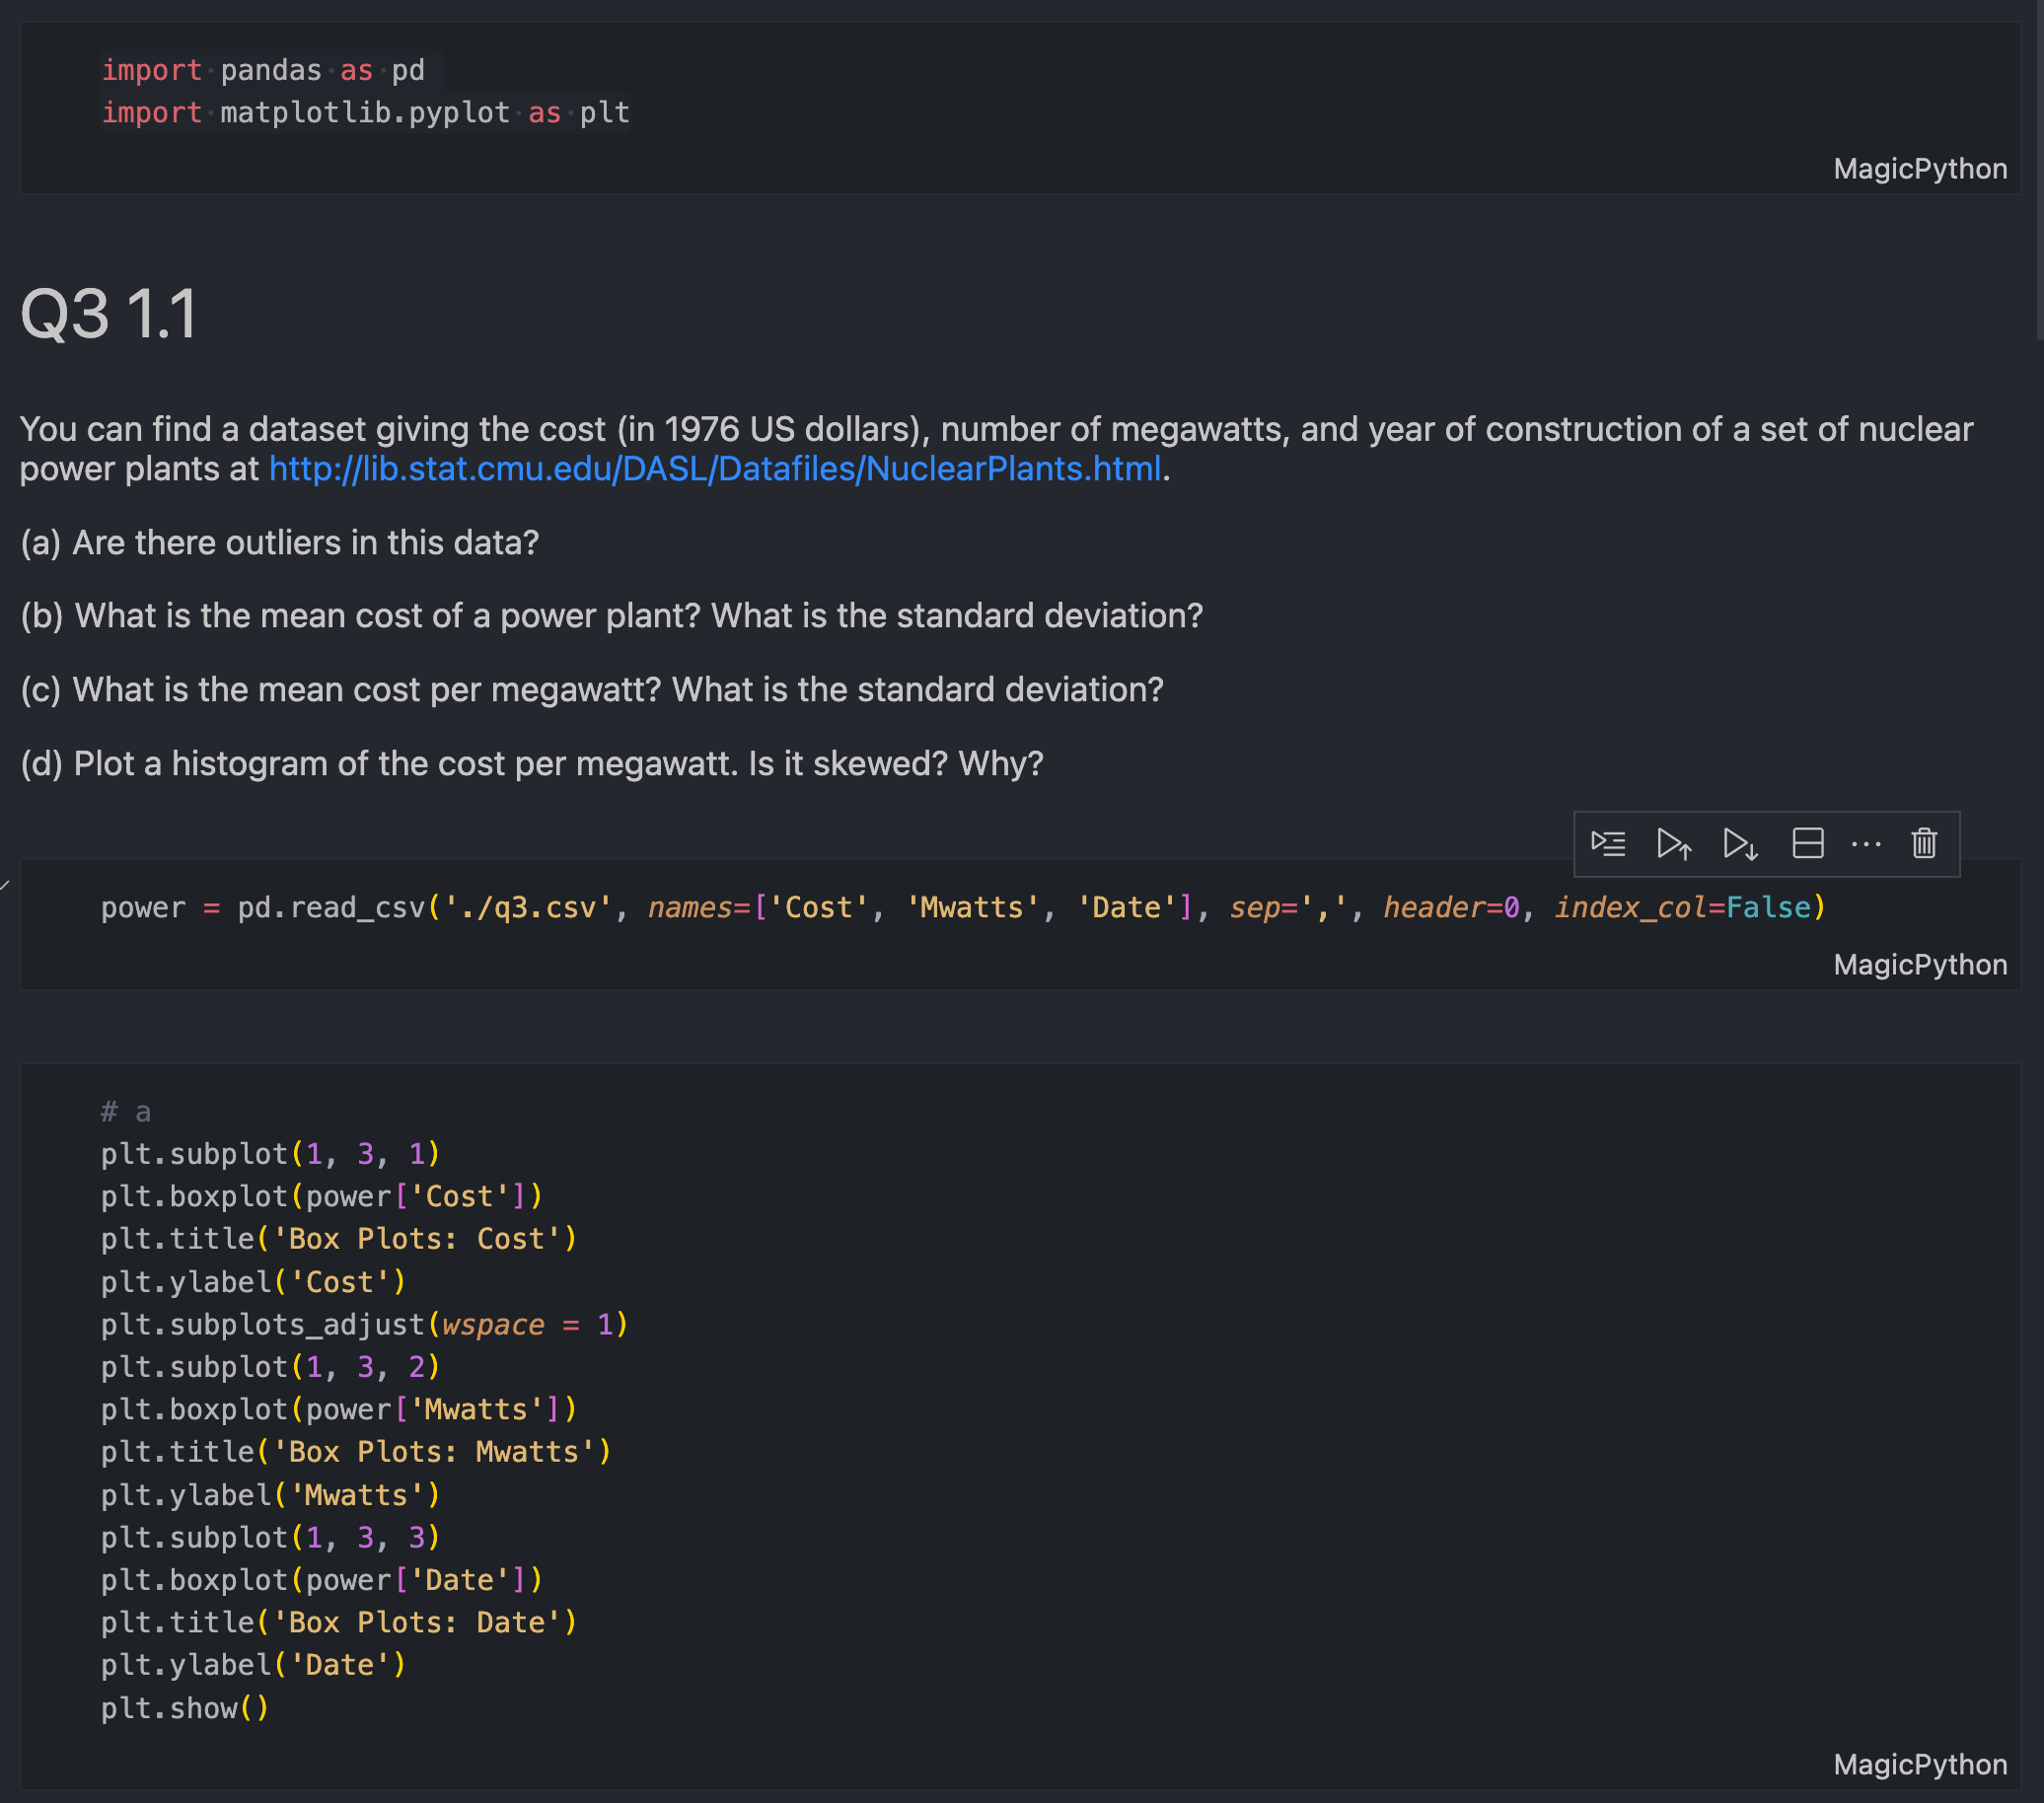
\includegraphics[scale=0.3]{q3a.png} 

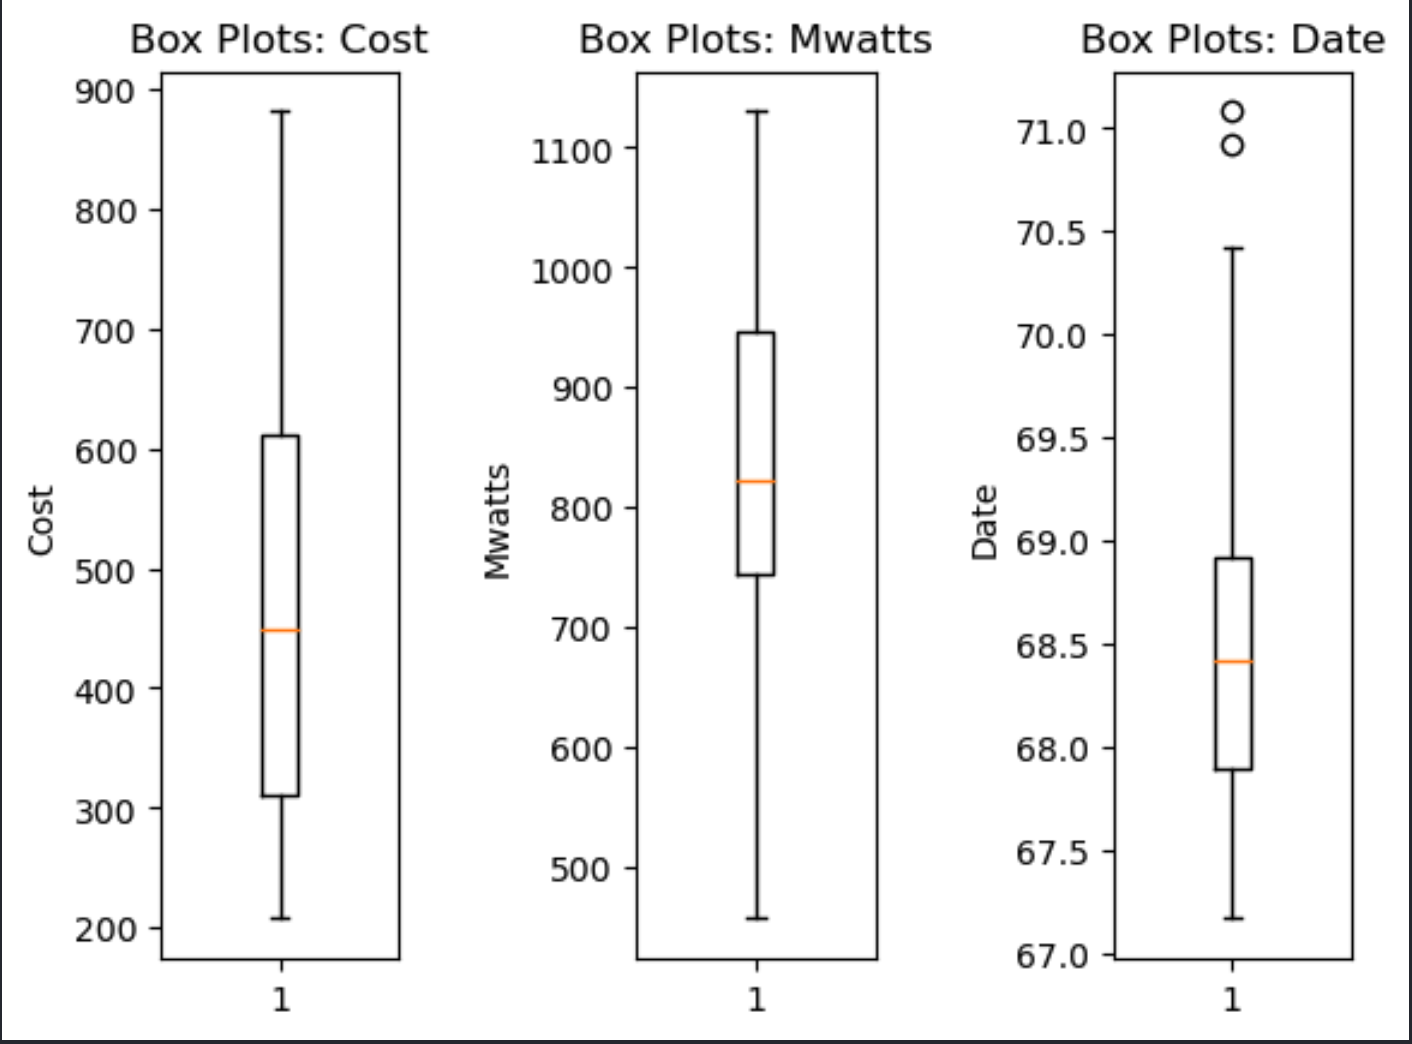
\includegraphics[scale=0.3]{q3a_plot.png}
\par
}
\begin{enumerate}[(a)]
    \item According the 3 box plots above, we can see that the ``Blot Plots: Date'' have two dots outside the range of the box and bracket. This means that there are 2 outliers in the data set. The other graphs doesn't contain any dots outside thus there are no outliers.
    \item \begin{verbatim}
        print(power.mean(axis=0))
        print(power.std(axis=0))
    \end{verbatim}
    Using the code above we can get the mean and standard deviation of each column of the data set. The result for cost is: 
    \begin{verbatim}
        ---mean---
        Cost      $ 461.560313 
        ---standard deviation---
        Cost      $ 170.120670
    \end{verbatim}
    \item By dividing the cost by the power we can get the cost per watt. Using this code:
    \begin{verbatim}
        print("---mean cost per megawatts---")
        power['costPerW'] = (power['Cost']/power['Mwatts'])
        print(power.mean(axis=0))
        print("---std cost per megawatts---")
        print(power.std(axis=0))
    \end{verbatim}
    The result is:
    \begin{verbatim}
        ---mean cost per megawatts---
        costPerW      $ 0.569735 per megawatts
        ---std cost per megawatts---
        costPerW      $ 0.187124 per megawatts
    \end{verbatim}
    \item The cost per megawatts is left skewed. This is because the mean is less than the median. The mean is 0.569735 and the median is 0.57957. Notice the mean line (red dashed line) is on the left of the median line (green dashed line) in the graph below.

    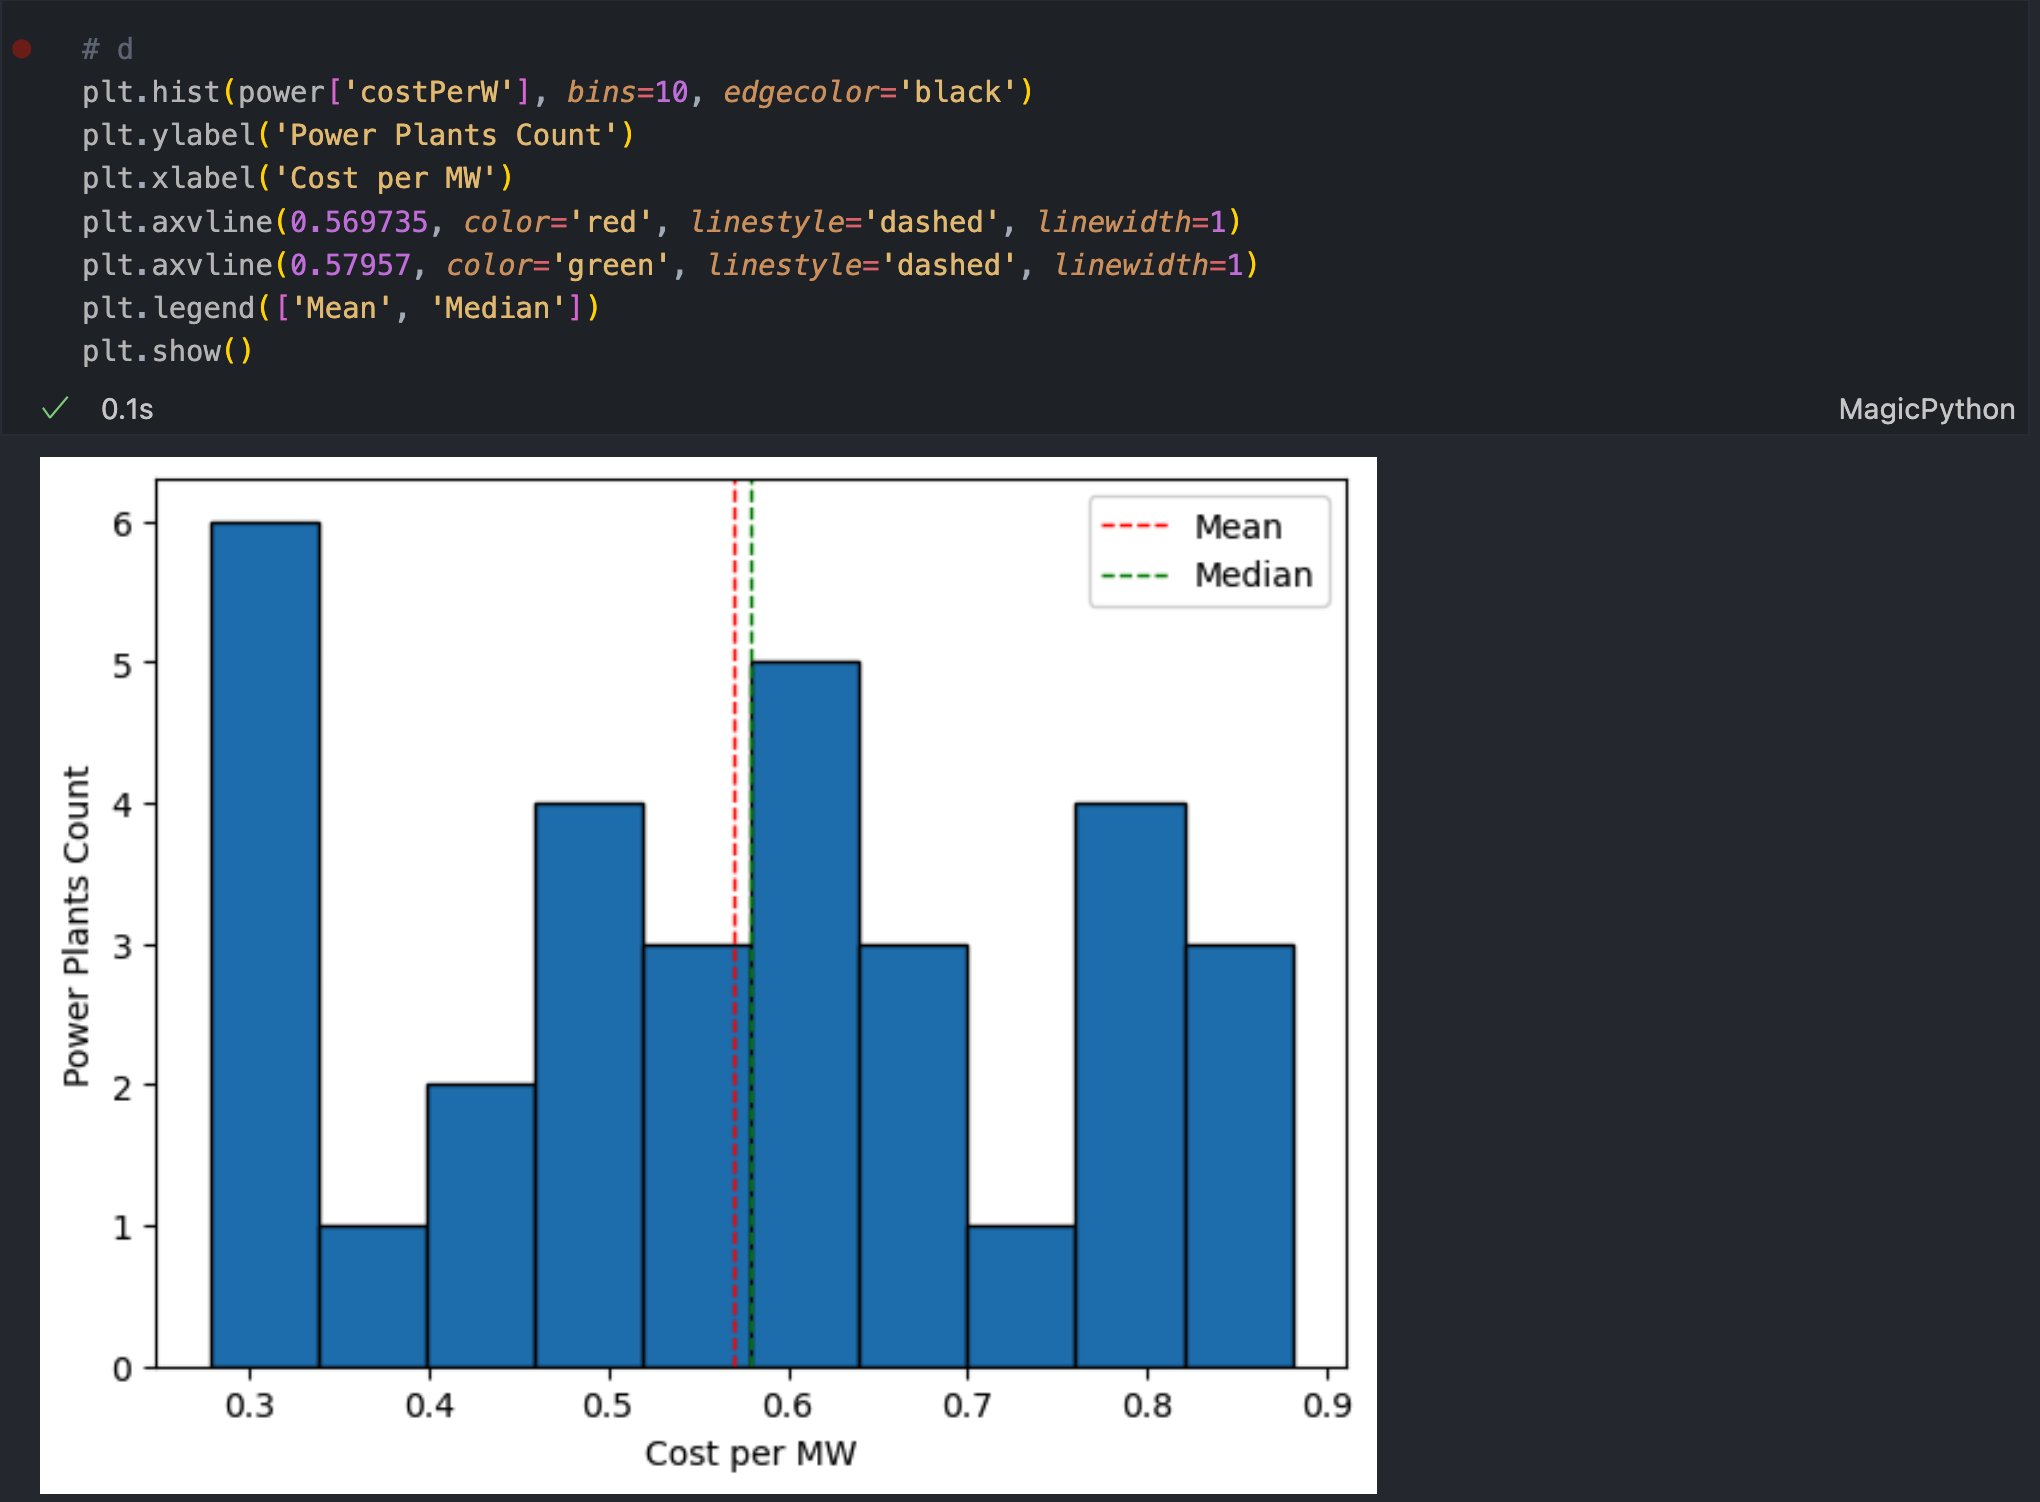
\includegraphics[scale=0.35]{q3d.png}

\end{enumerate}

\newpage

\section*{Question 4}
    \includegraphics*[scale=0.4]{q4.png}
    
    \includegraphics*[scale=0.3]{q4_plot1.png}
    \includegraphics*[scale=0.3]{q4_plot2.png}

    The above code generates 2 of the histogram graphs. The one of the left show calories count in each food category and the one on the right show the sodium count in each food category. 
    

    \null By looking at the left graph, we can clearly see that many of the poultry food (orange) have the lowest calories count than the other food categories. The beef(blue) and meat(green) have similarly higher calories.

    By looking at the right graph, we can see that the sodium count in each food category is very similar. The poultry(orange) have the highest sodium count spike, the beef(blue) have the lowest sodium count spike. The meet(green) have the second highest sodium count.

\newpage

\section*{Question 5}

    The code below plot a box plot showing the statistic of three or more syllable for each magazine group.

    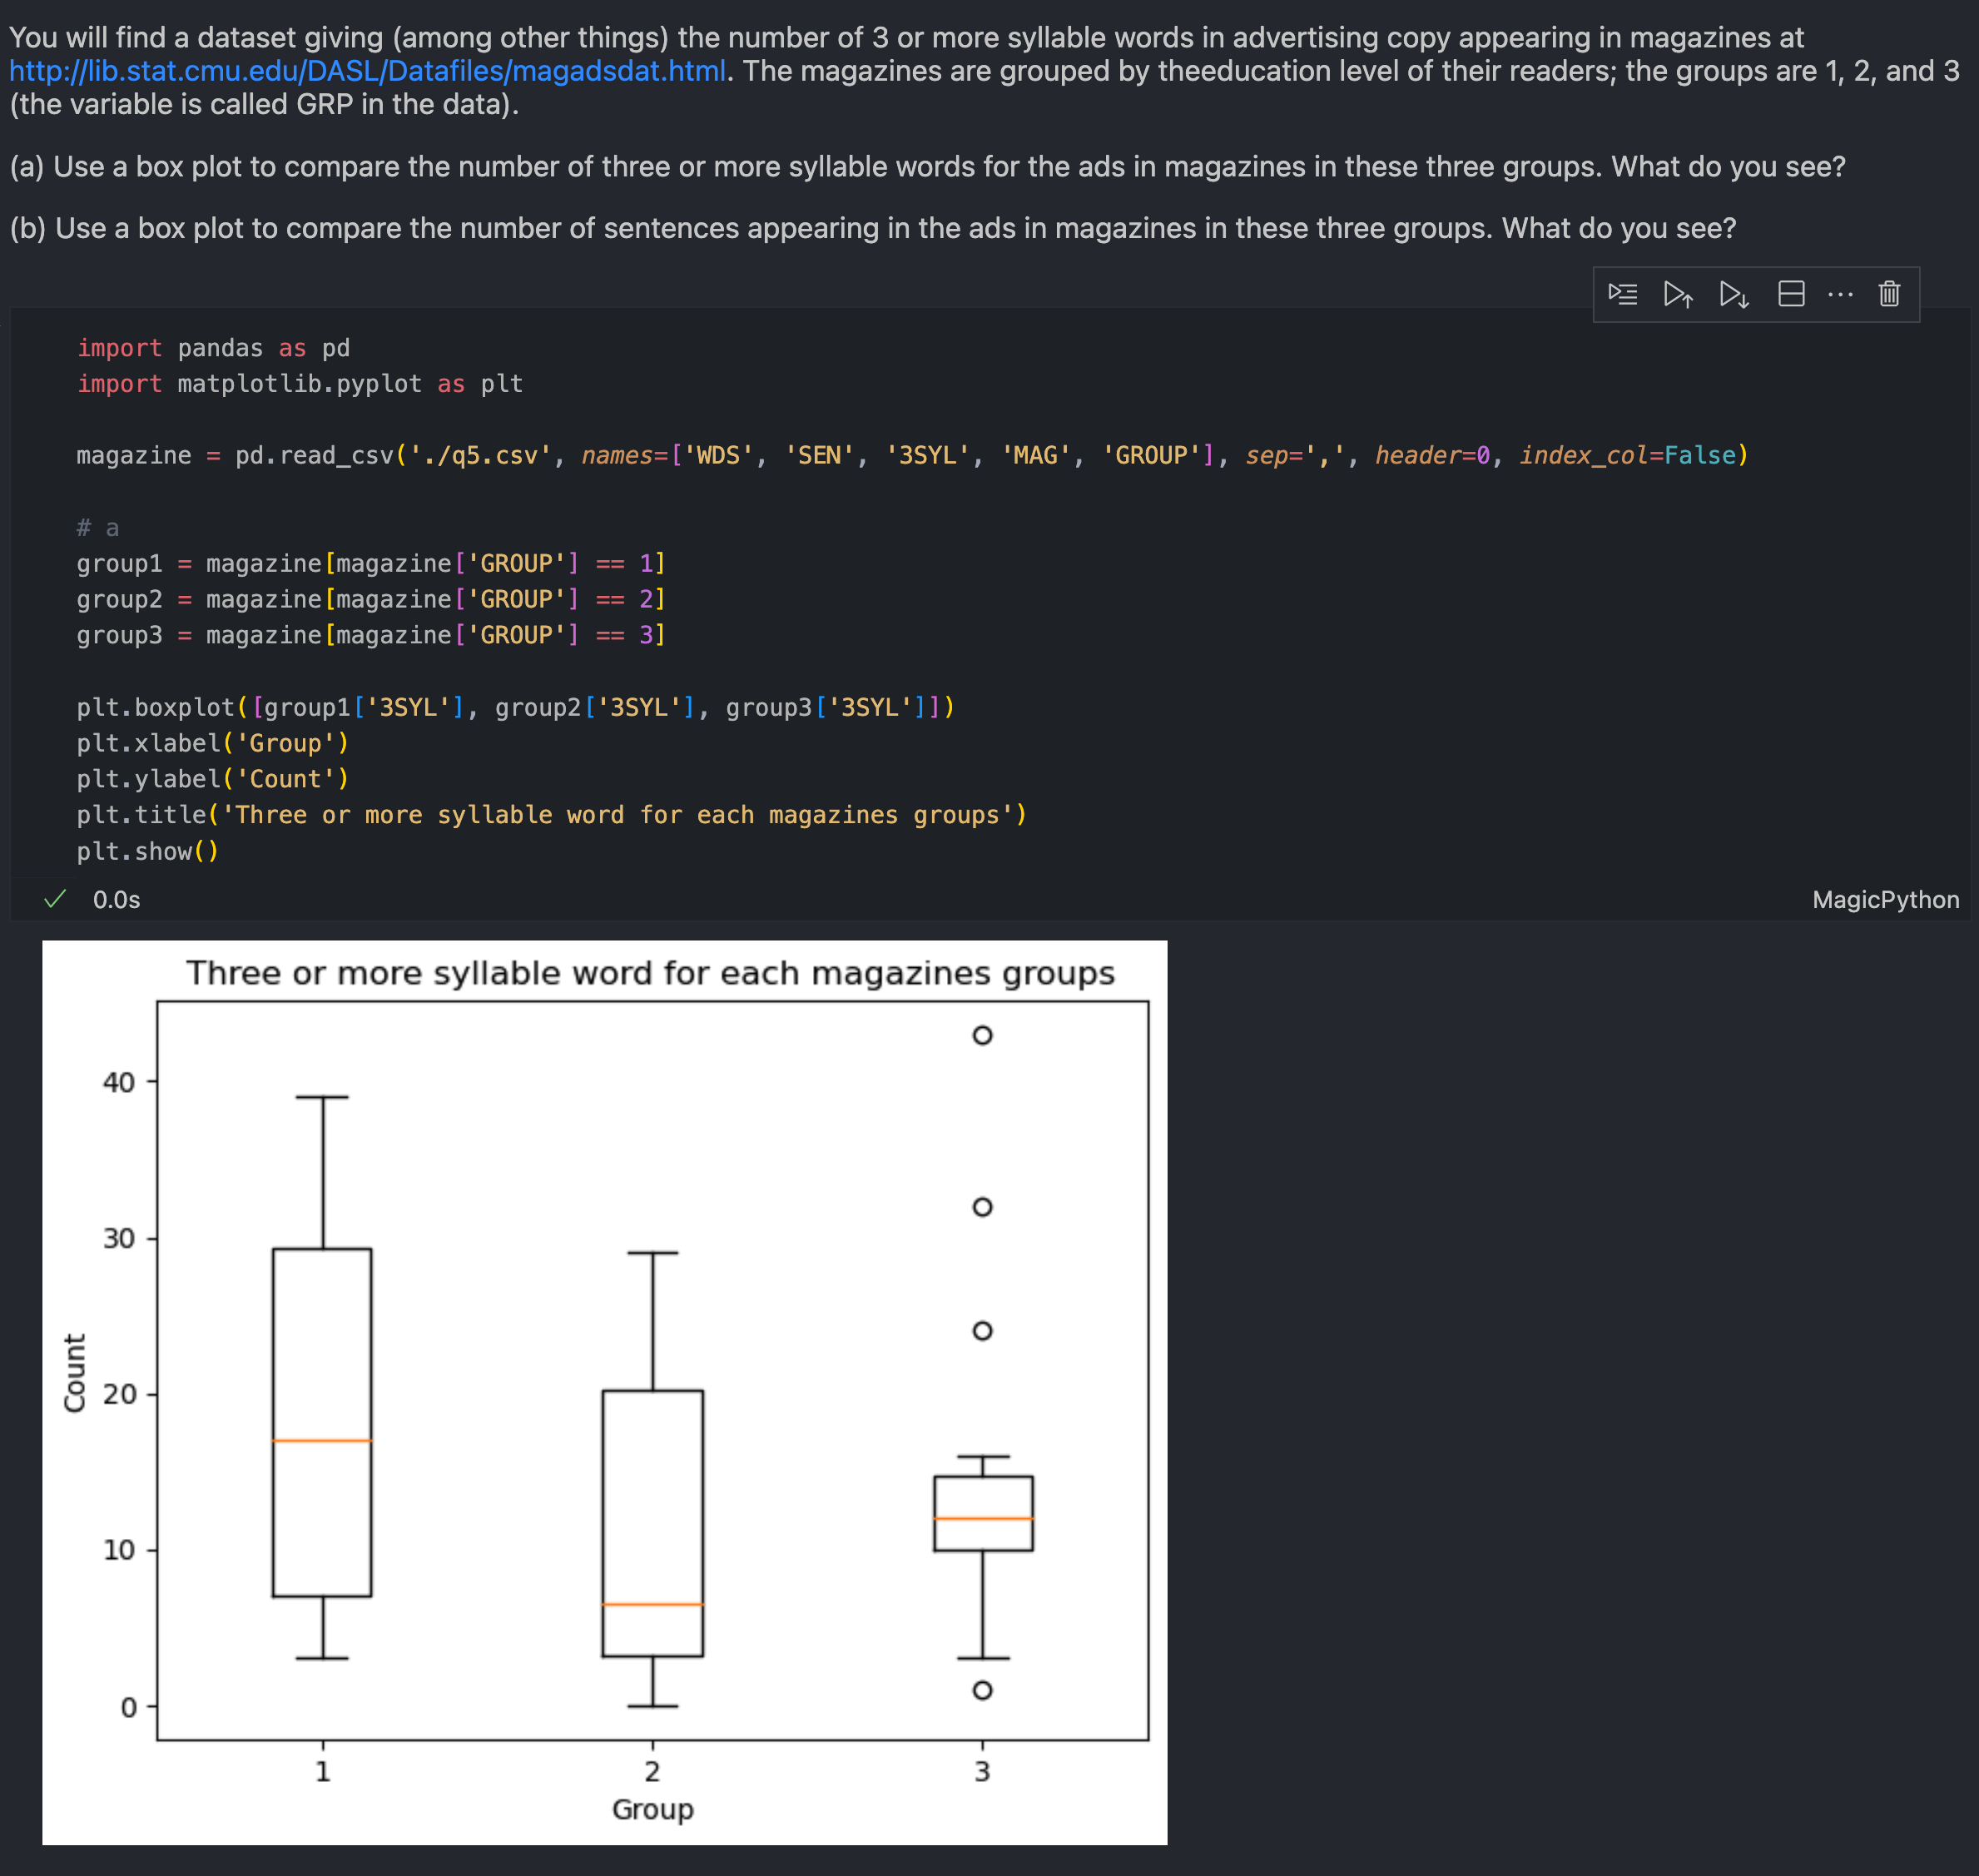
\includegraphics[scale=0.35]{q5a.png} 

    
    (a) Looking at the box plot we can notice that the median for the amount of three or more syllable word for each group are arrange from least to greatest as follows: 2, 3, 1.
    One major difference in the groups can be seen in magazine group 3. It has the significantly lower interquartile range compared to other and there are 4 outliers data in this group.

    \newpage
    The code below plot a box plot showing the statistic of number of sentences for each magazine group.

    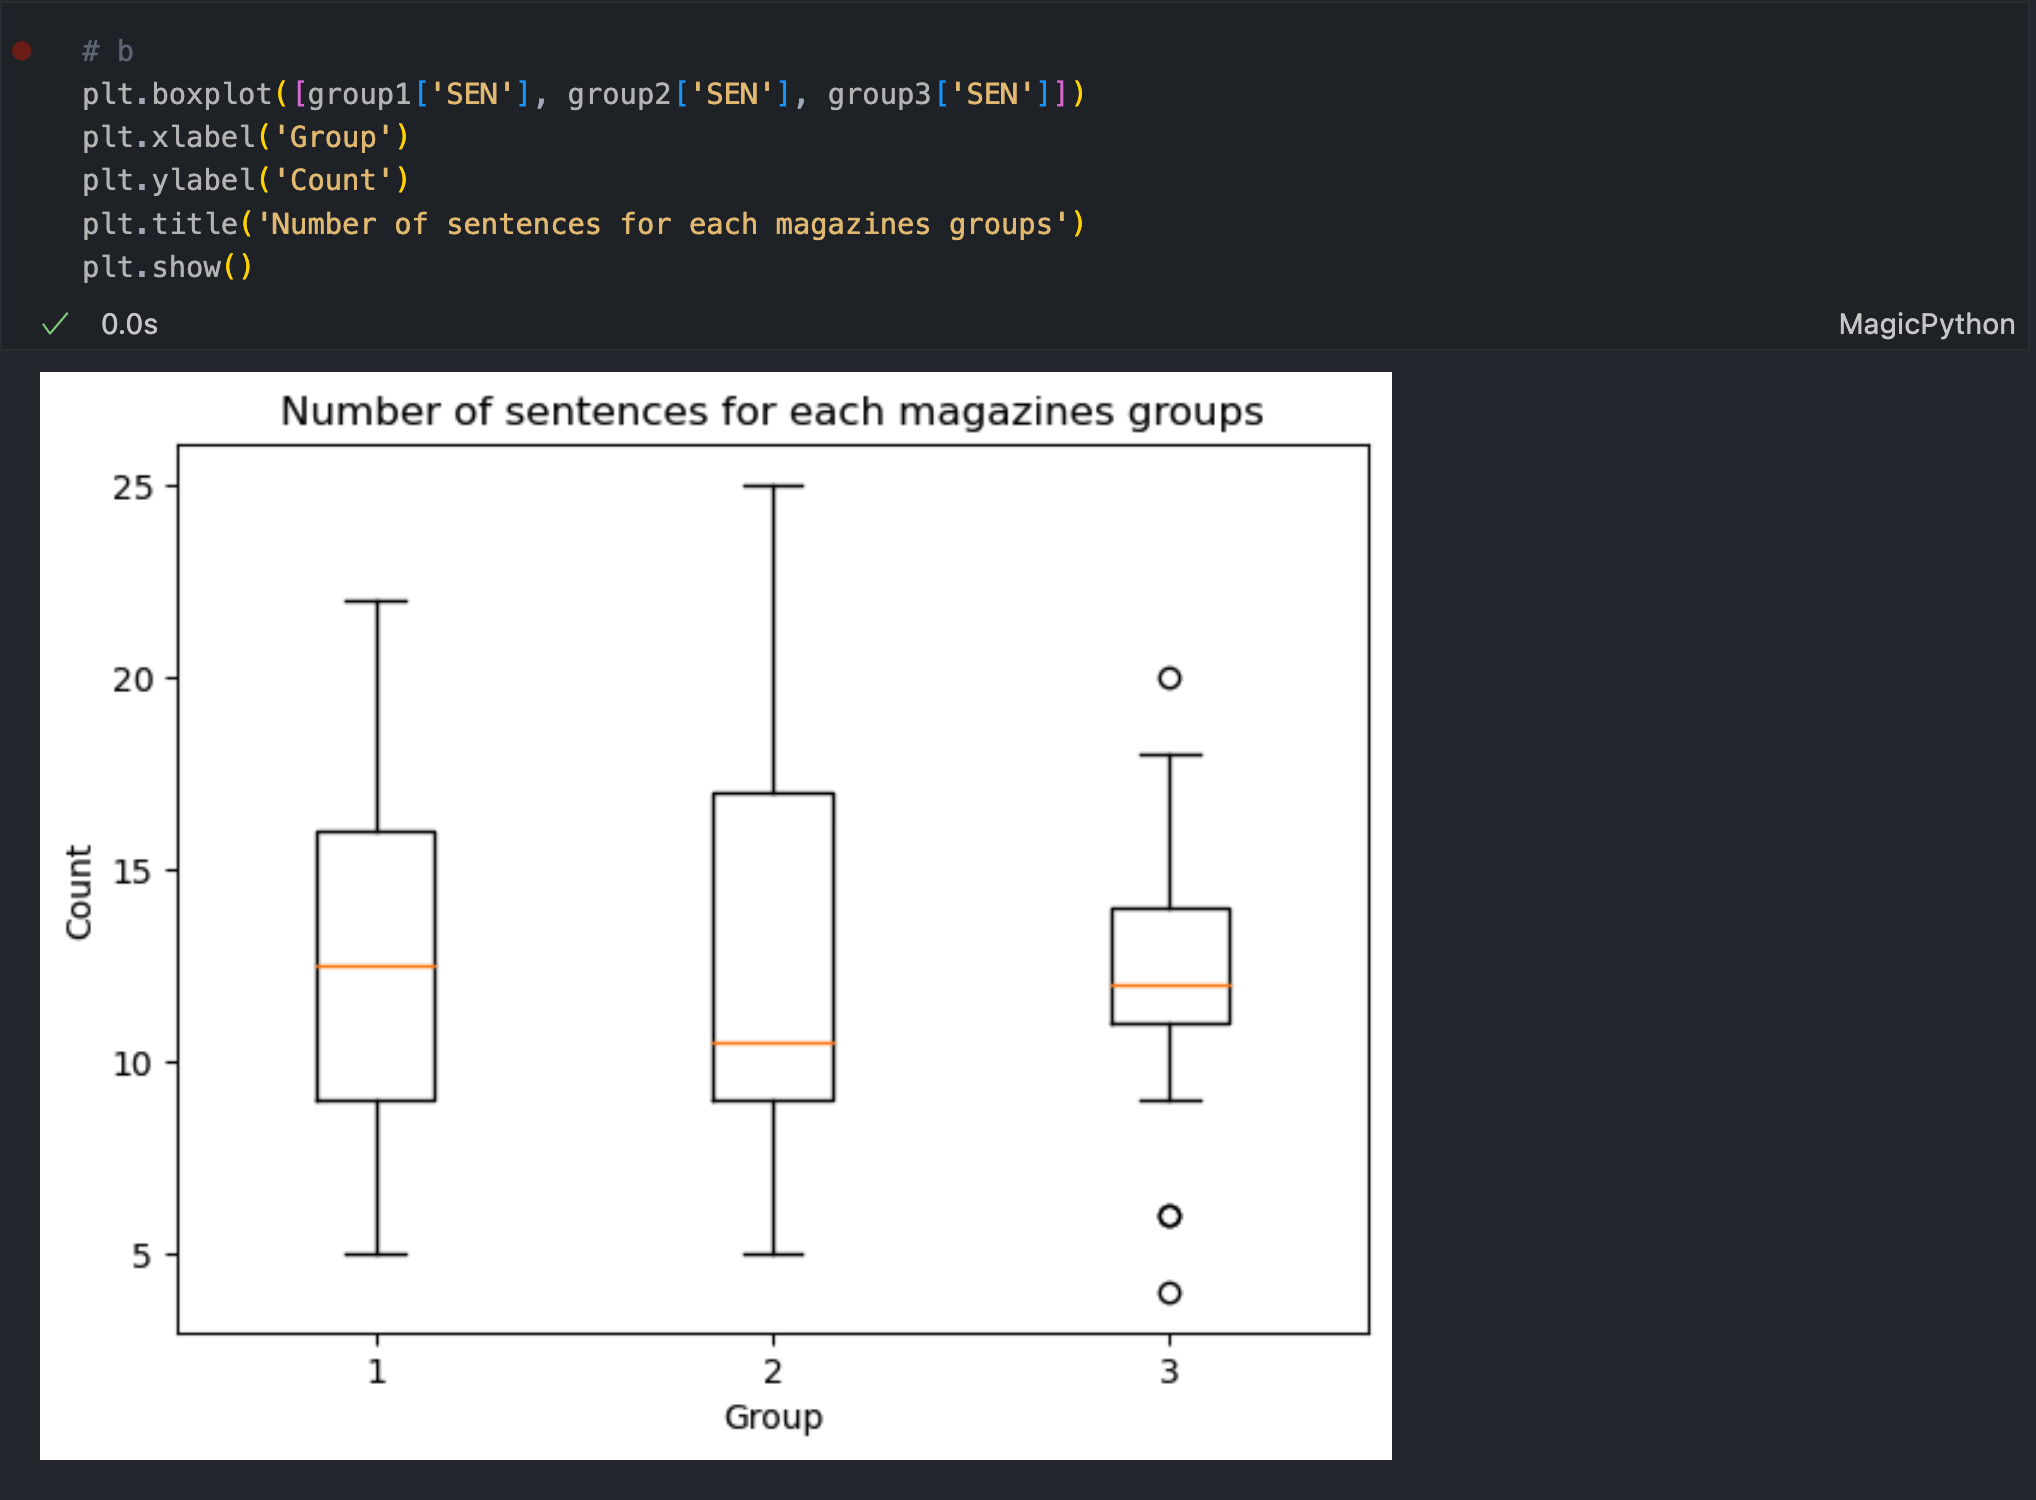
\includegraphics[scale=0.35]{q5b.png}

    (b) Looking at the box plot we can notice that the median for the amount of sentences for each group are arrange from least to greatest as follows: 2, 3, 1.
    One major difference in the groups can be seen in magazine group 3. It has the significantly lower interquartile range compared to other and there are 3 outliers data in this group.

\newpage

\section*{Question 6}

(Extra credit 5 points) Let $\{x_i\}$
 be a dataset consisting of $N$
 real numbers, $x_1,...,x_N$
. Prove the function $g(m)=\sum_{i=1}^{N}|(x_i-m)|$
 is minimized when $m=median(\{x_i\})$
. Hint: try to prove $(\sum_{i=1}^{N}|(x_i-d)|)-(\sum_{i=1}^{N}|(x_i-median)|)\geq0$
 for $d \geq median$
, then for $d \leq median$
, d is any real number.


Let $\{x_i\}$ be a dataset consisting of $N$ real numbers, $x_1,...,x_N$. Prove the function $g(m)=\sum_{i=1}^{N}|(x_i-m)|$ is minimized when $m=median(\{x_i\})$. Hint: try to prove $(\sum_{i=1}^{N}|(x_i-d)|)-(\sum_{i=1}^{N}|(x_i-median)|)\geq0$ for $d \geq median$, then for $d \leq median$, d is any real number.

\subsection*{Answer}

\qquad First, consider the inequality $(\sum_{i=1}^{N} |x_i - d| - \sum_{i=1}^{N} |x_i - median| \geq 0)$ for $(d \geq median)$.
\newline

We break it into cases based on whether $(x_i)$ is less than or greater than the median, and note that the sum on the left side is larger than or equal to the sum on the right side.
\newline

Extending this argument to $(d \leq median)$, we find that the same inequality holds.
\newline

In both cases, the function $(g(m))$ can't be minimized with $(m)$ away from the median, as moving $(m)$ towards the median reduces the left-hand side of the inequality. Therefore, $(g(m))$ is minimized when $(m = median(\{x_i\}))$. 

\end{document}
